\documentclass{beamer}

\usepackage{paratype}
\setbeamerfont{frametitle}{family=\bf}
\usepackage{listings}
\usepackage{pdfpages}
\usepackage{verbatim}

\lstset{
  language=C,
  keepspaces=true,
  moredelim=**[is][\color{red}]{@}{@},
}

% Beamer theme settings
\usecolortheme{seagull}
\usenavigationsymbolstemplate{} % no navigation buttons

\usepackage[utf8]{inputenc}

\title{OpenCL day 1: GPU hardware and the programming model}

\author{Cosmin Oancea and Troels Henriksen}

\date{January 28, 2019}

\begin{document}

\frame{\titlepage}

\section{Introduction and Course Contents}

\begin{frame}
  \tableofcontents[currentsection]
\end{frame}

\section{Hardware Trends}

\begin{frame}
	\tableofcontents[currentsection]
\end{frame}

\begin{frame}
  \frametitle{The first computers were not this}

  \begin{center}
    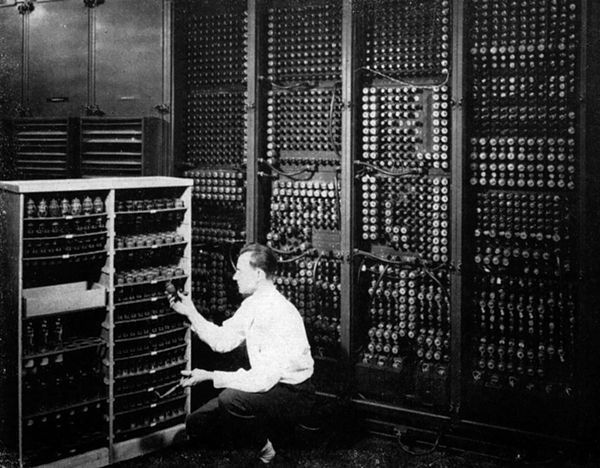
\includegraphics[width=\textwidth]{img/eniac.jpg}
  \end{center}

\end{frame}

\begin{frame}
  \frametitle{But this}

  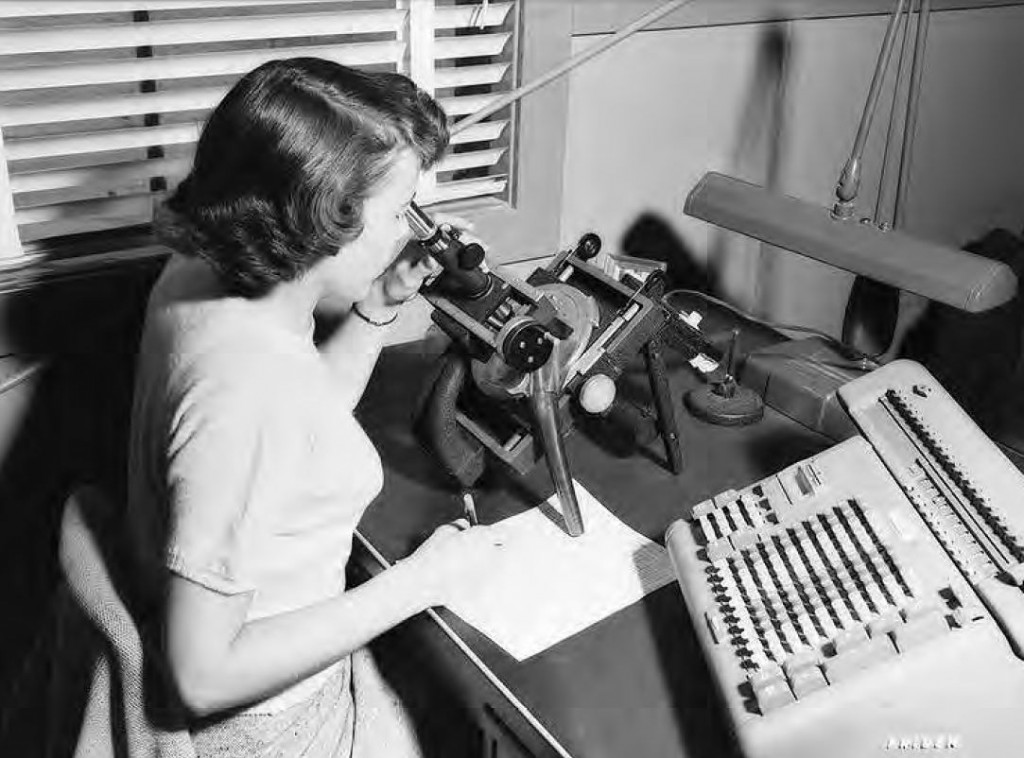
\includegraphics[width=\textwidth]{img/human-computer.jpg}
\end{frame}

\begin{frame}
  \frametitle{And if you had a larger problem}

  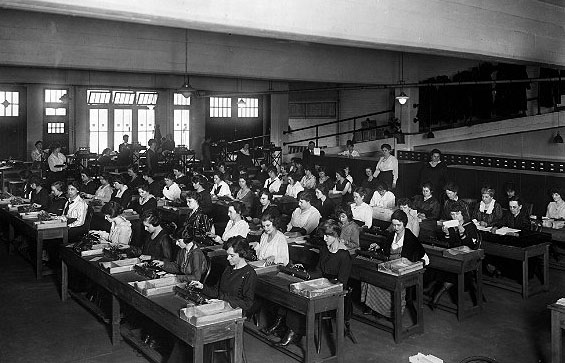
\includegraphics[width=\textwidth]{img/human-computers.jpg}
\end{frame}

\begin{frame}
  \frametitle{But then they started looking like this}

  \begin{center}
    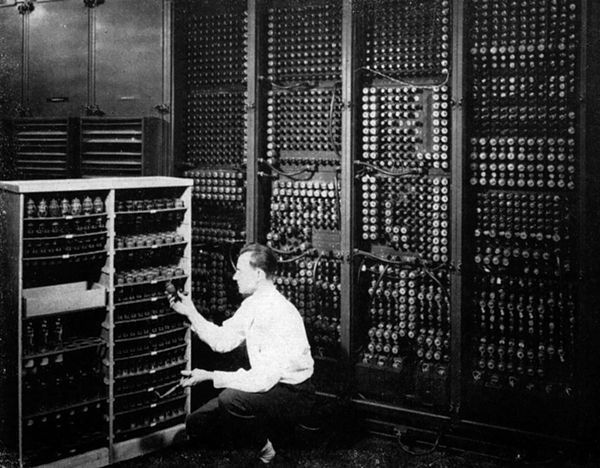
\includegraphics[width=\textwidth]{img/eniac.jpg}
  \end{center}
\end{frame}

\begin{frame}
  \frametitle{Then this}
  \begin{center}
    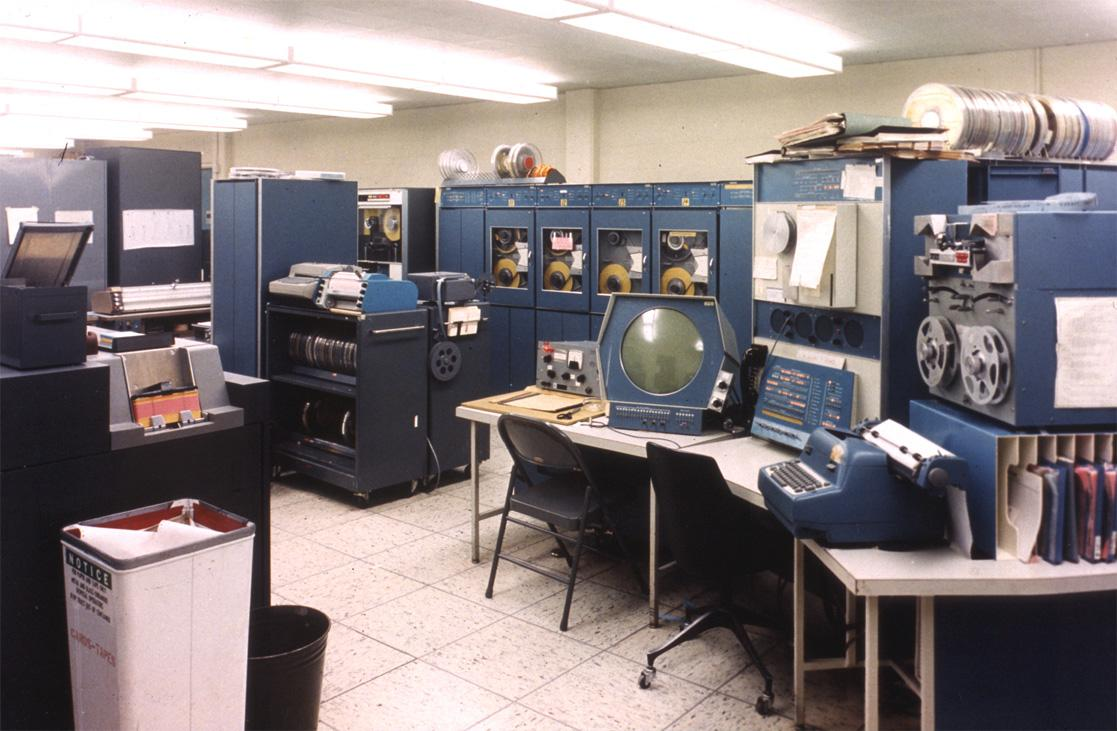
\includegraphics[width=\textwidth]{img/pdp1.jpg}
  \end{center}
\end{frame}

\begin{frame}
  \frametitle{Then this}
  \begin{center}
    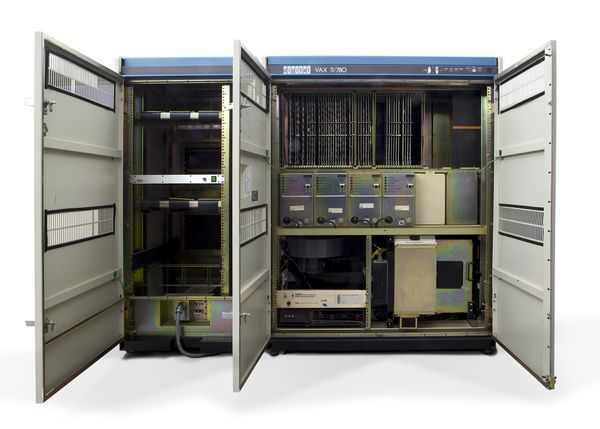
\includegraphics[width=\textwidth]{img/vax.jpg}
  \end{center}
\end{frame}

\begin{frame}
  \frametitle{Then this}
  \begin{center}
    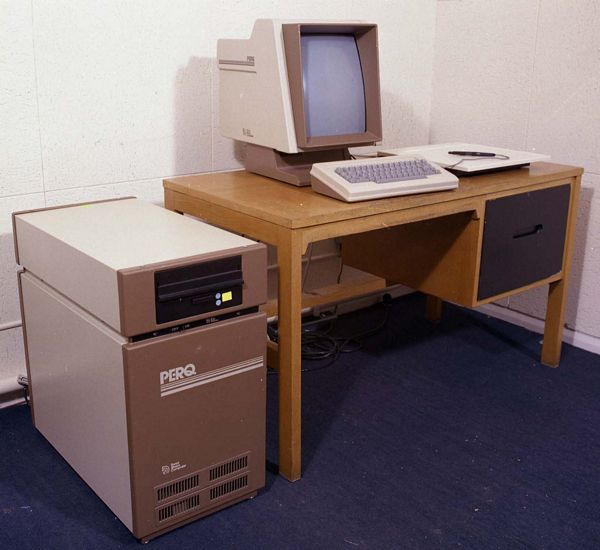
\includegraphics[width=\textwidth]{img/early-workstation.jpg}
  \end{center}
\end{frame}

\begin{frame}
  \frametitle{Then this}
  \begin{center}
    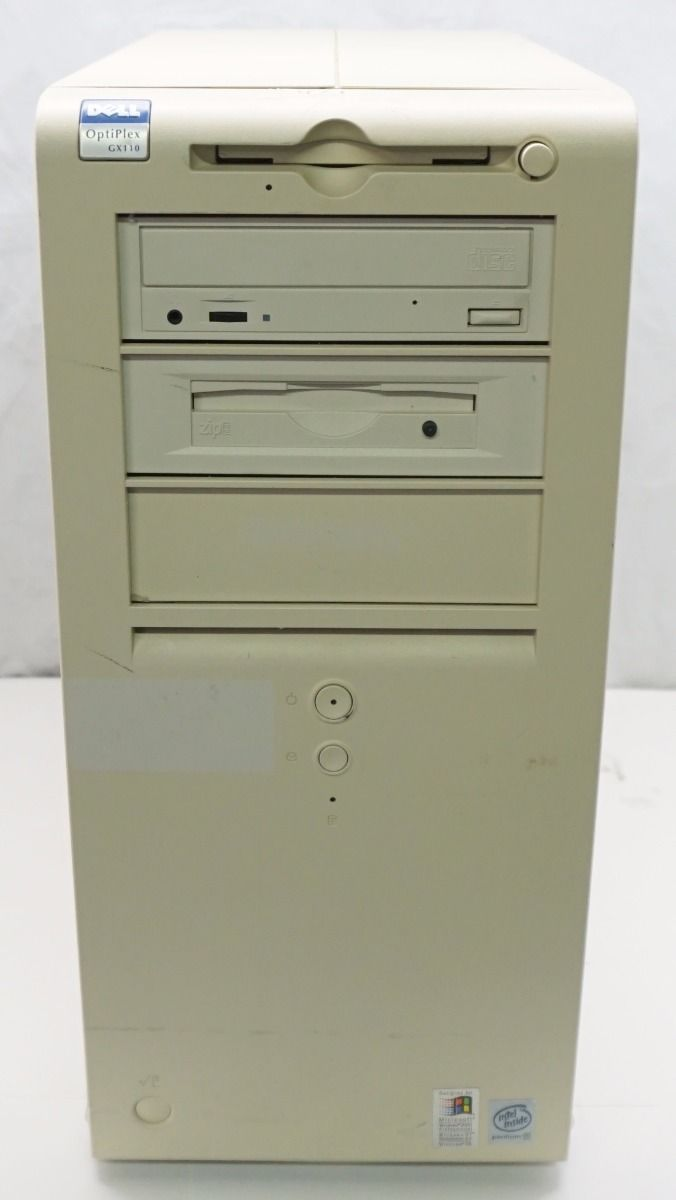
\includegraphics[width=\textwidth]{img/dell.jpg}
  \end{center}
\end{frame}

\begin{frame}
  \frametitle{Then this}
  \begin{center}
    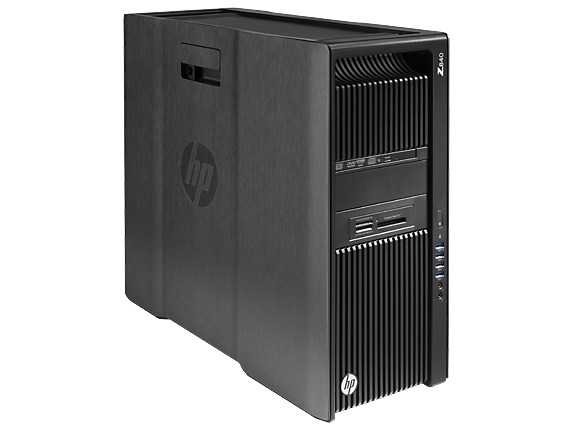
\includegraphics[width=\textwidth]{img/hp.jpg}
  \end{center}
\end{frame}

\begin{frame}
  \frametitle{Then, from around 2005}
  \begin{center}
    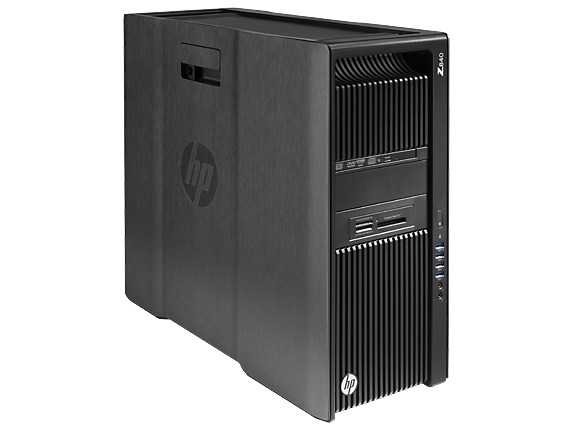
\includegraphics[width=0.5\textwidth]{img/hp.jpg}
    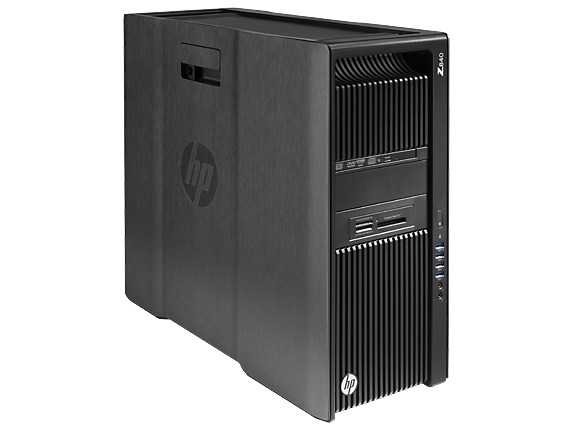
\includegraphics[width=0.5\textwidth]{img/hp.jpg}
  \end{center}
\end{frame}

\begin{frame}
  \frametitle{Then, from around 2005}
  \begin{center}
    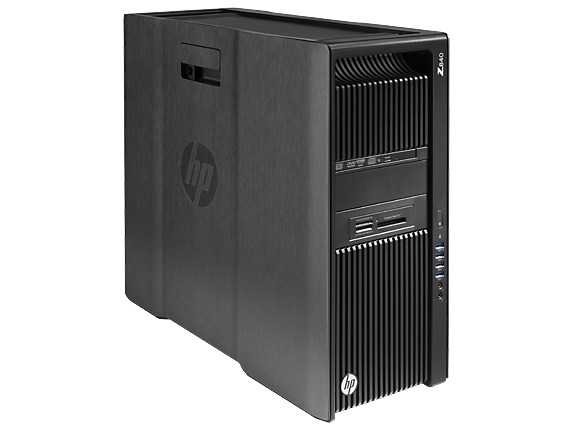
\includegraphics[width=0.3\textwidth]{img/hp.jpg}
    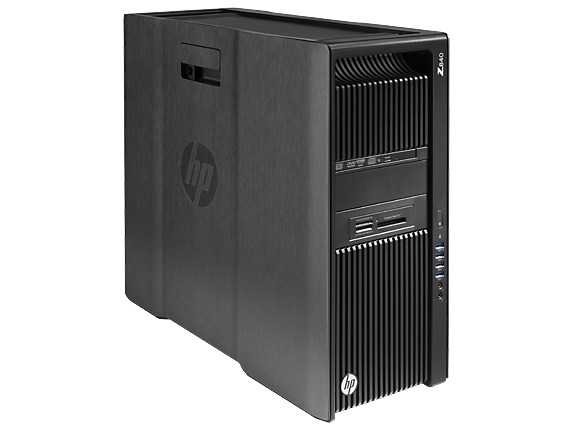
\includegraphics[width=0.3\textwidth]{img/hp.jpg}
    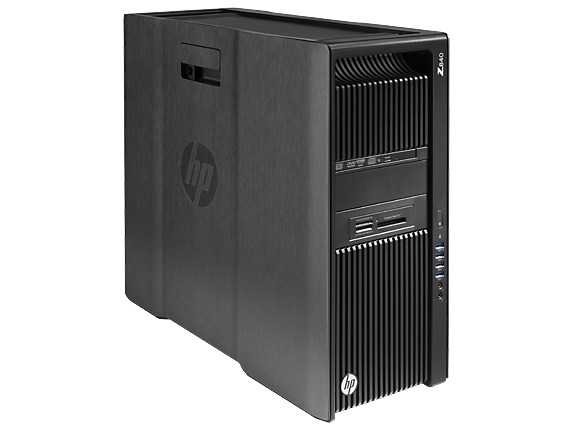
\includegraphics[width=0.3\textwidth]{img/hp.jpg}
  \end{center}

\end{frame}

\begin{frame}
  \frametitle{Then, from around 2005}
  \begin{center}
    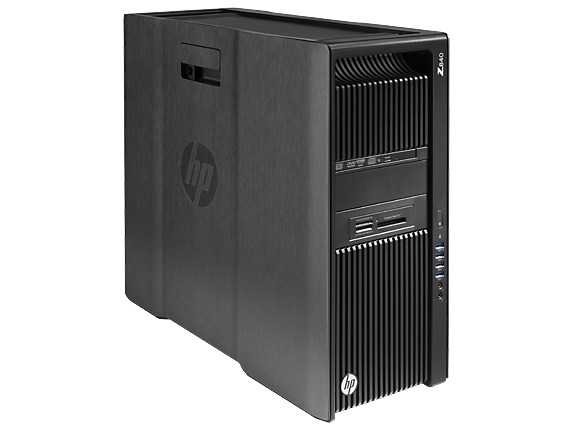
\includegraphics[width=0.3\textwidth]{img/hp.jpg}
    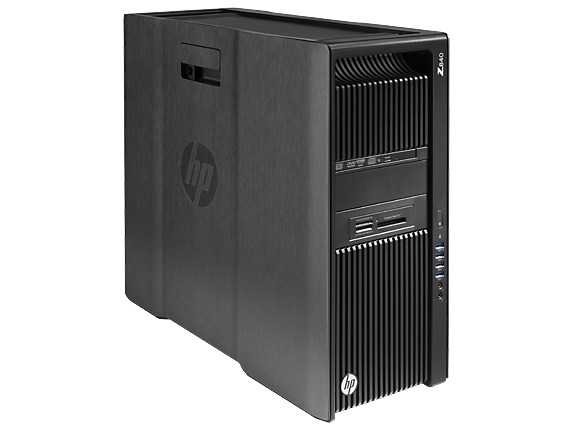
\includegraphics[width=0.3\textwidth]{img/hp.jpg}
    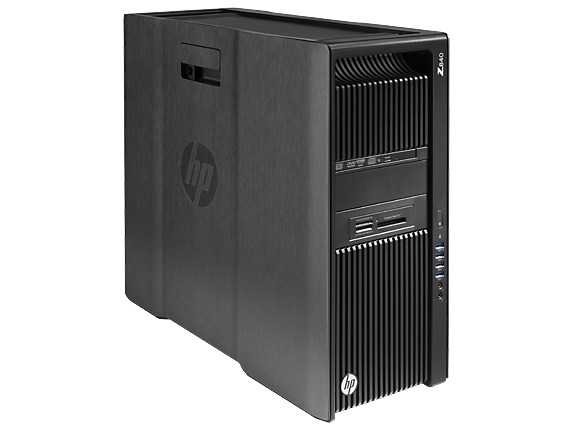
\includegraphics[width=0.3\textwidth]{img/hp.jpg}

    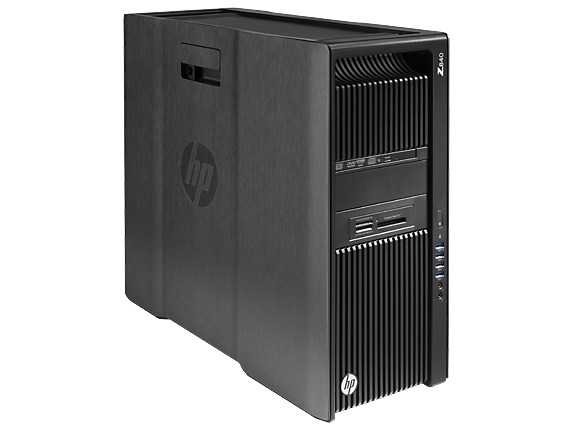
\includegraphics[width=0.3\textwidth]{img/hp.jpg}
    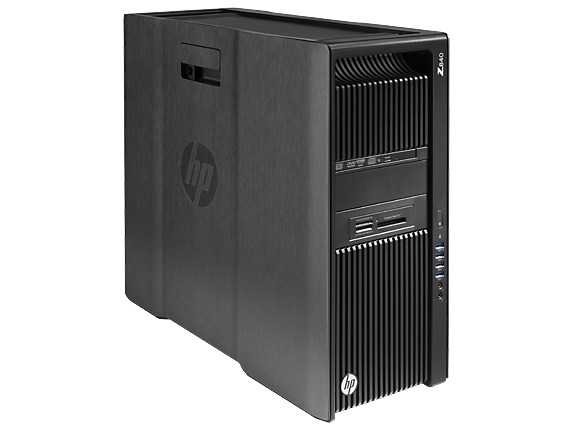
\includegraphics[width=0.3\textwidth]{img/hp.jpg}
    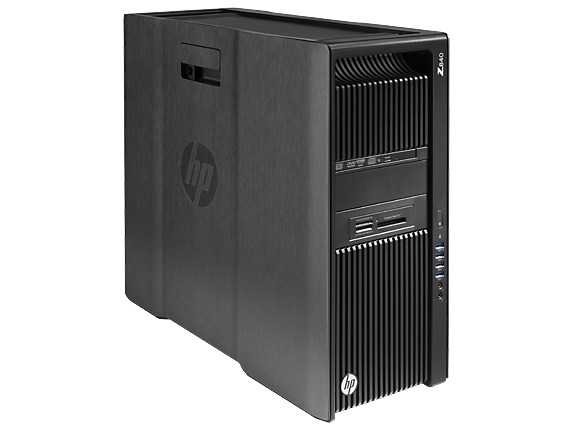
\includegraphics[width=0.3\textwidth]{img/hp.jpg}
  \end{center}

  Improvements in \textit{sequential performance} stalled, although
  computers still got smaller and faster.
\end{frame}

\begin{frame}
  \frametitle{What Changed?}

  \begin{itemize}
  \item \textit{Power complexity} $P_{dynamic} \sim Freq^3$,
    preventing us from increasing processor frequency.
  \item \textit{Memory wall}, ever-increasing performance gap between
    processor and memory (which means that \textit{memory} becomes
    bottleneck, not processor speed).
  \end {itemize}
\end{frame}

\begin{frame}
  \frametitle{CPU progress}

  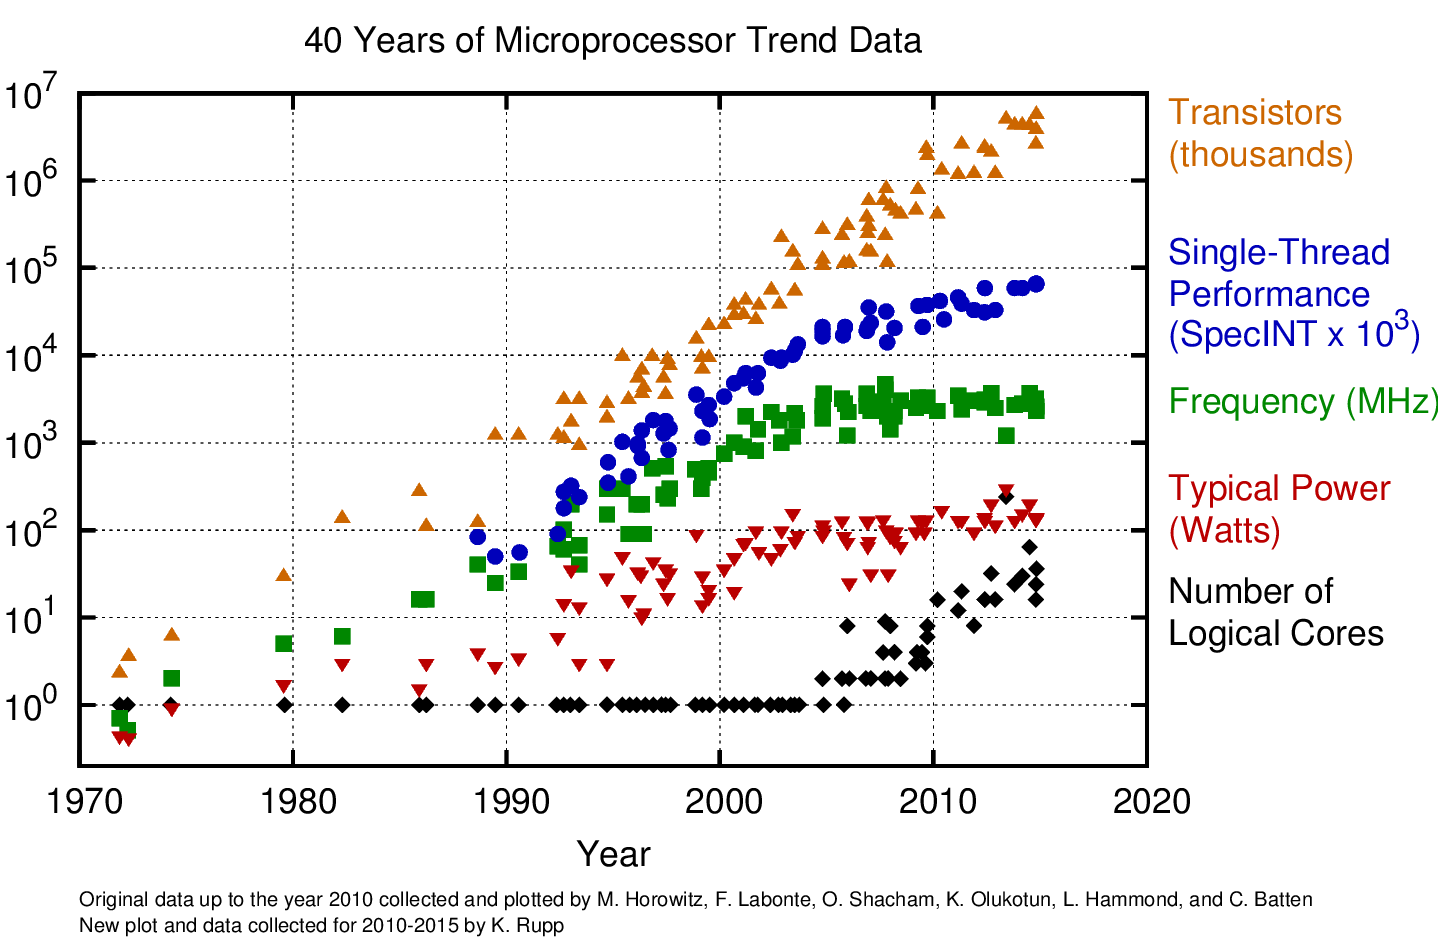
\includegraphics[width=\textwidth]{img/40-years-processor-trend.png}

Addressed with \textit{more cores}.

\end{frame}

\begin{frame}
  \frametitle{The Memory Wall}

\begin{center}
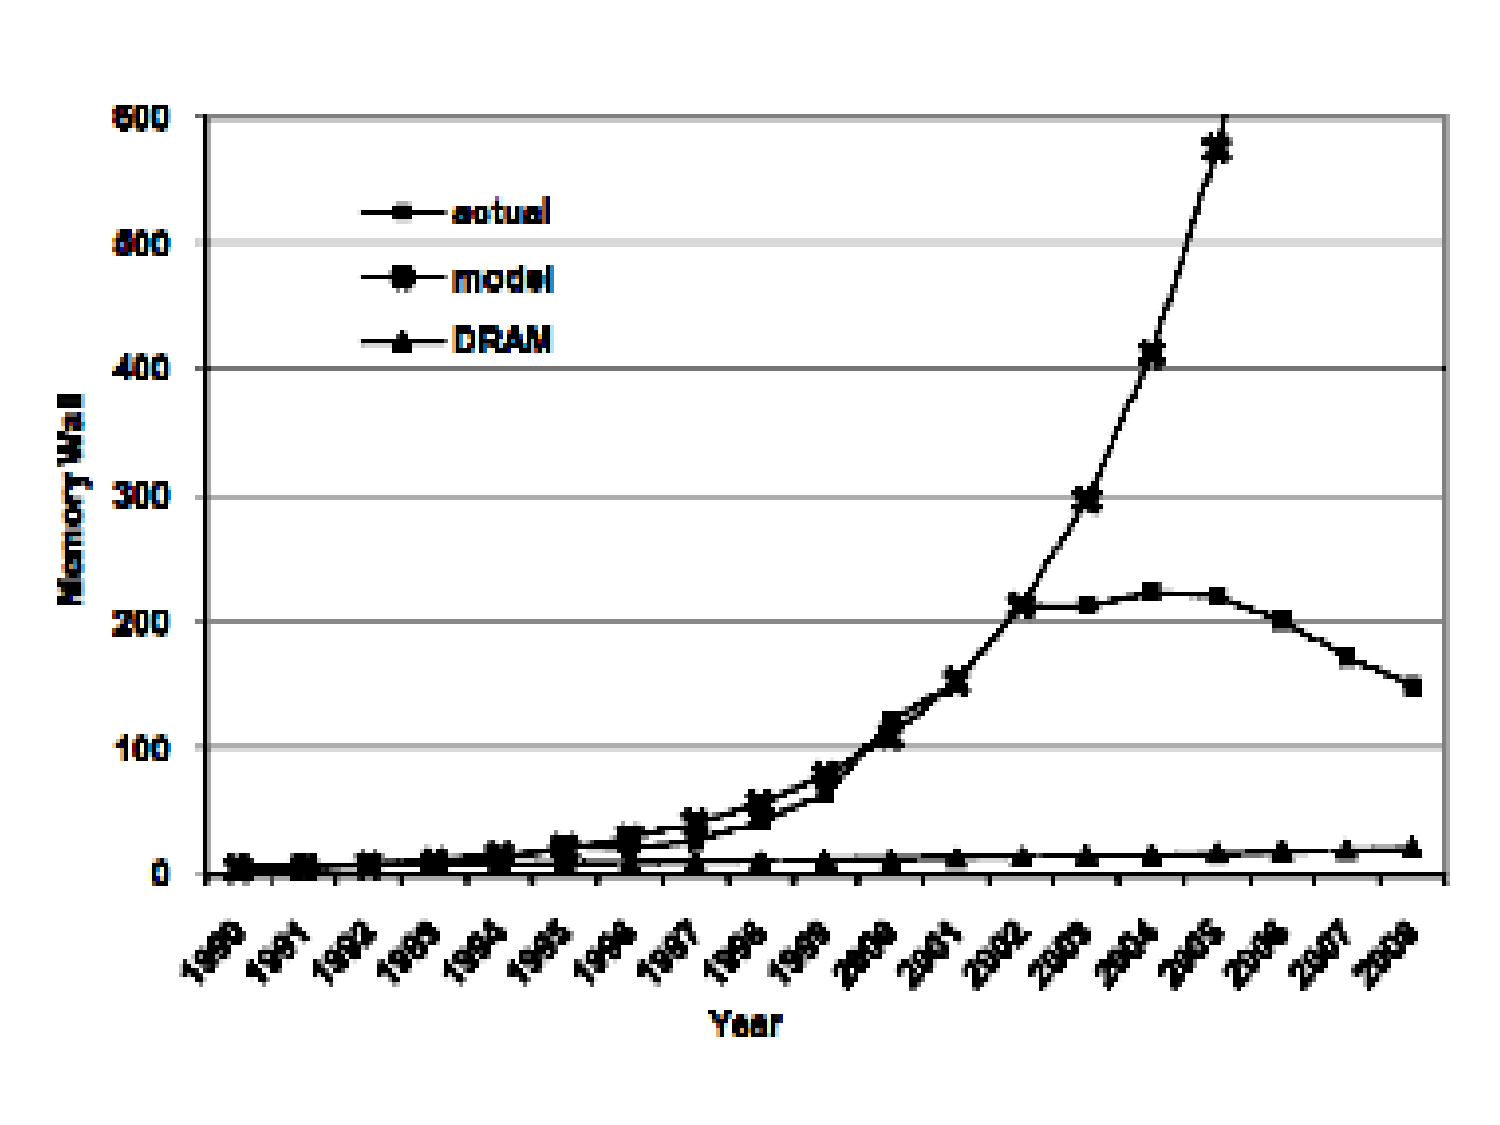
\includegraphics[width=50ex]{img/memwall}

  Memory Wall = $\text{processor cycles} / \text{memory cycles}$
\end{center}

Addressed with caches (not scalable) and \textit{latency hiding}.

\end{frame}

\begin{frame}
  \frametitle{This is why GPUs are useful}

  The design of GPUs directly attacks these two problems.

  \begin{itemize}
  \item\textbf{Frequency scaling} becomes less of an issue because we
    can instead use thousands of (slower) cores.

  \item The \textbf{memory wall} is partially circumvented by using
    faster and smaller memory, but mostly by \textit{latency hiding}.
    With tens of thousands of threads, we can probably find something
    else to do while some threads are waiting for memory!
  \end{itemize}

  Ultimately, GPUs do \textit{throughput processing}, and operations
  have (relatively) high latency.

\end{frame}

\begin{frame}
  \frametitle{CPUs compared to CPUs}

  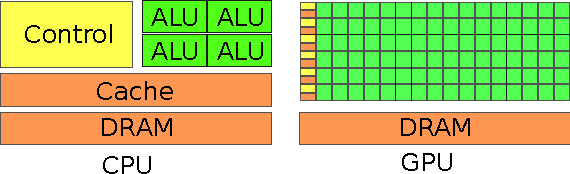
\includegraphics[width=\textwidth]{img/cpu-gpu-architecture.pdf}

  \begin{itemize}
  \item GPUs have \textit{thousands} of simple cores and taking full
    advantage of their compute power requires \textit{tens of
      thousands} of threads.
  \item GPU threads are very \textit{restricted} in what they can do:
    no stack, no allocation, limited control flow, etc.
  \item Potential \textit{very high performance} and \textit{lower
      power usage} compared to CPUs, but programming them is
    \textit{hard}.
  \end{itemize}

\end{frame}

\begin{frame}[fragile,t]
\frametitle{GPUs and Memory}

\begin{center}
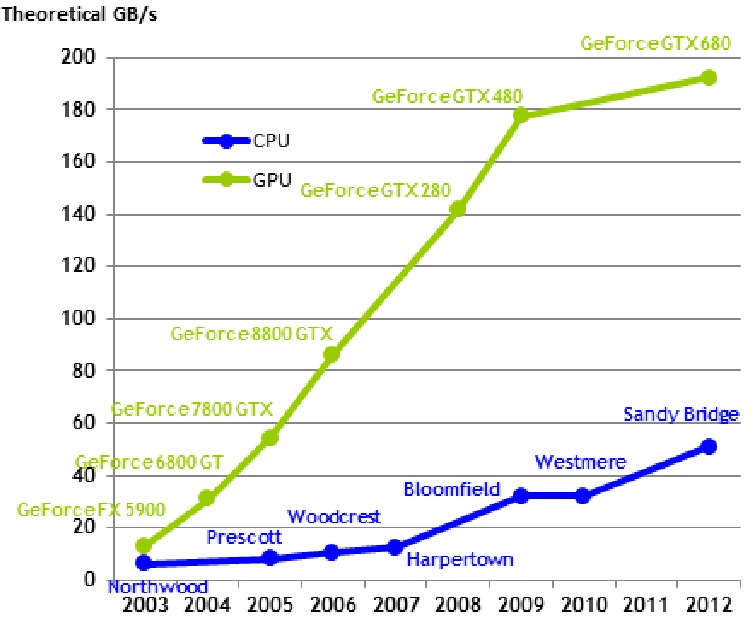
\includegraphics[height=45ex]{img/gpubandwidth.png}
\end  {center}

\end{frame}

\begin{frame}[fragile,t]
\frametitle{GPUs and GFLOPS}

\begin{center}
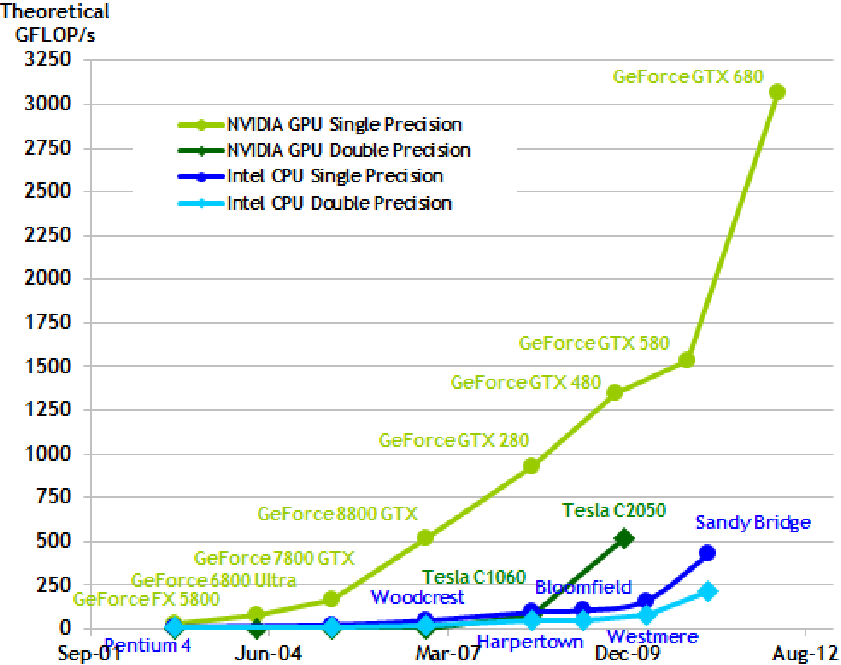
\includegraphics[height=43ex]{img/gpugflops.png}
\end  {center}

\end{frame}


\section{The GPU Architecture}

\begin{frame}
	\tableofcontents[currentsection]
\end{frame}

\begin{frame}
  The following slides are taken from the presentation
  \textit{Introduction to GPU Architecture} by Ofer Rosenberg of AMD.
\end{frame}

{
\setbeamercolor{background canvas}{bg=}
\includepdf[pages=4-38]{img/Introduction-to-GPUs.pdf}
}

\begin{frame}
  \frametitle{The GPU we will be using: Radeon HD
    7800\footnote{\url{https://developer.amd.com/wordpress/media/2012/12/AMD_Southern_Islands_Instruction_Set_Architecture.pdf}}}

  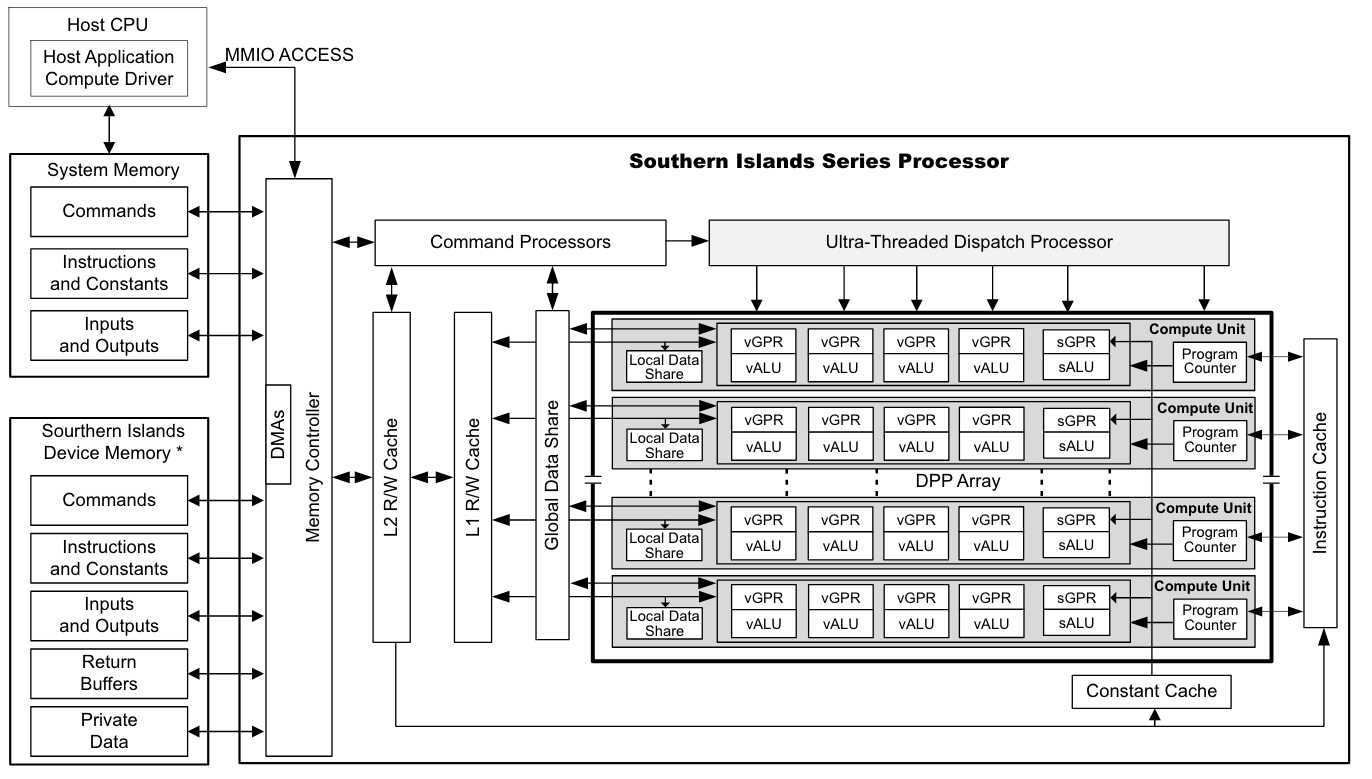
\includegraphics[width=\textwidth]{img/pitcairn.png}
\end{frame}

\begin{frame}
  \frametitle{Zooming in on the Compute Units}

  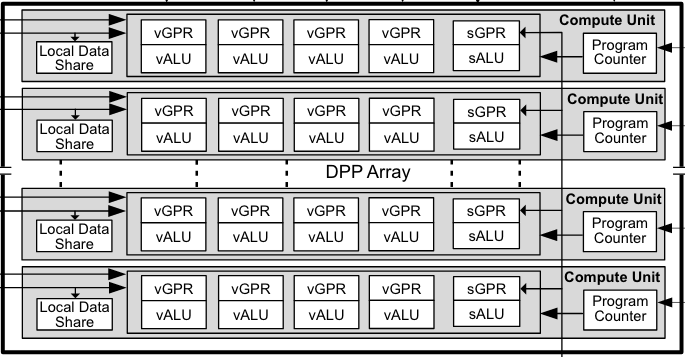
\includegraphics[width=\textwidth]{img/pitcairn-cus.png}

  \begin{itemize}
  \item Each vector-ALU executes a \textit{wavefront} of 64 work-items
    over four clock cycles.
  \item Many wavefronts in flight at once to hide latency.
  \end{itemize}

\end{frame}
\section{The OpenCL Programming Model}

\begin{frame}
	\tableofcontents[currentsection]
\end{frame}

\begin{frame}[fragile,t]
\frametitle{GPU programming}

\begin{center}
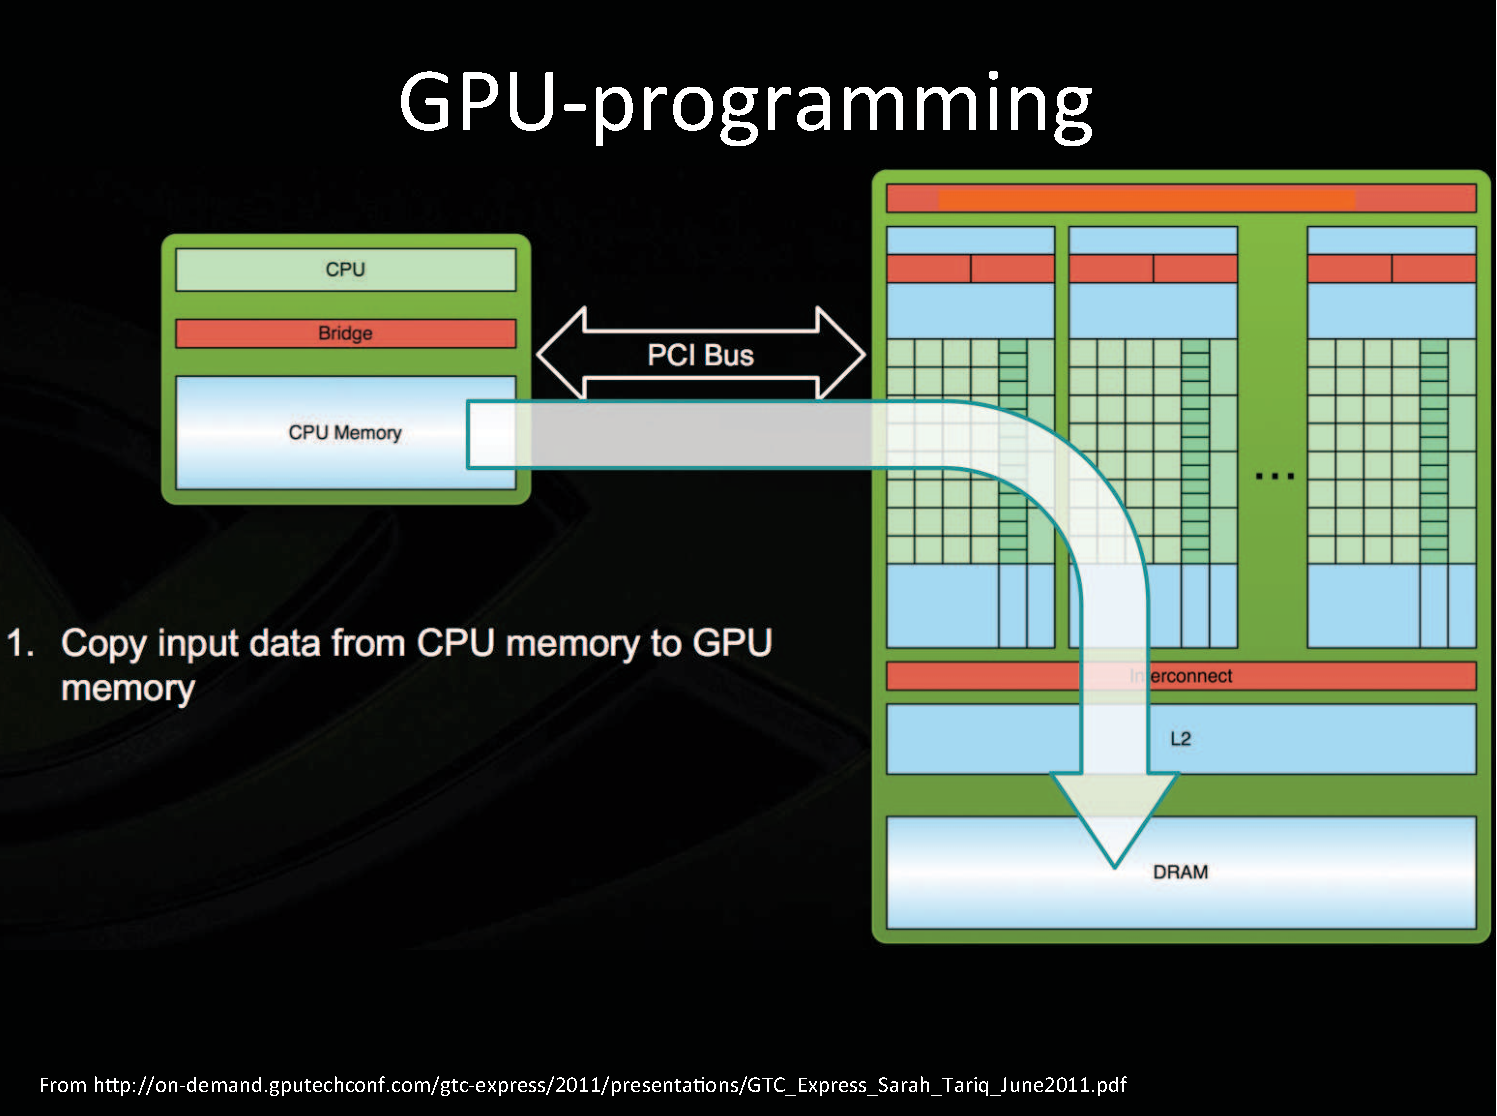
\includegraphics[height=43ex]{img/MemCpy1.pdf}
\end  {center}

\end{frame}

\begin{frame}[fragile,t]
\frametitle{GPU programming}

\begin{center}
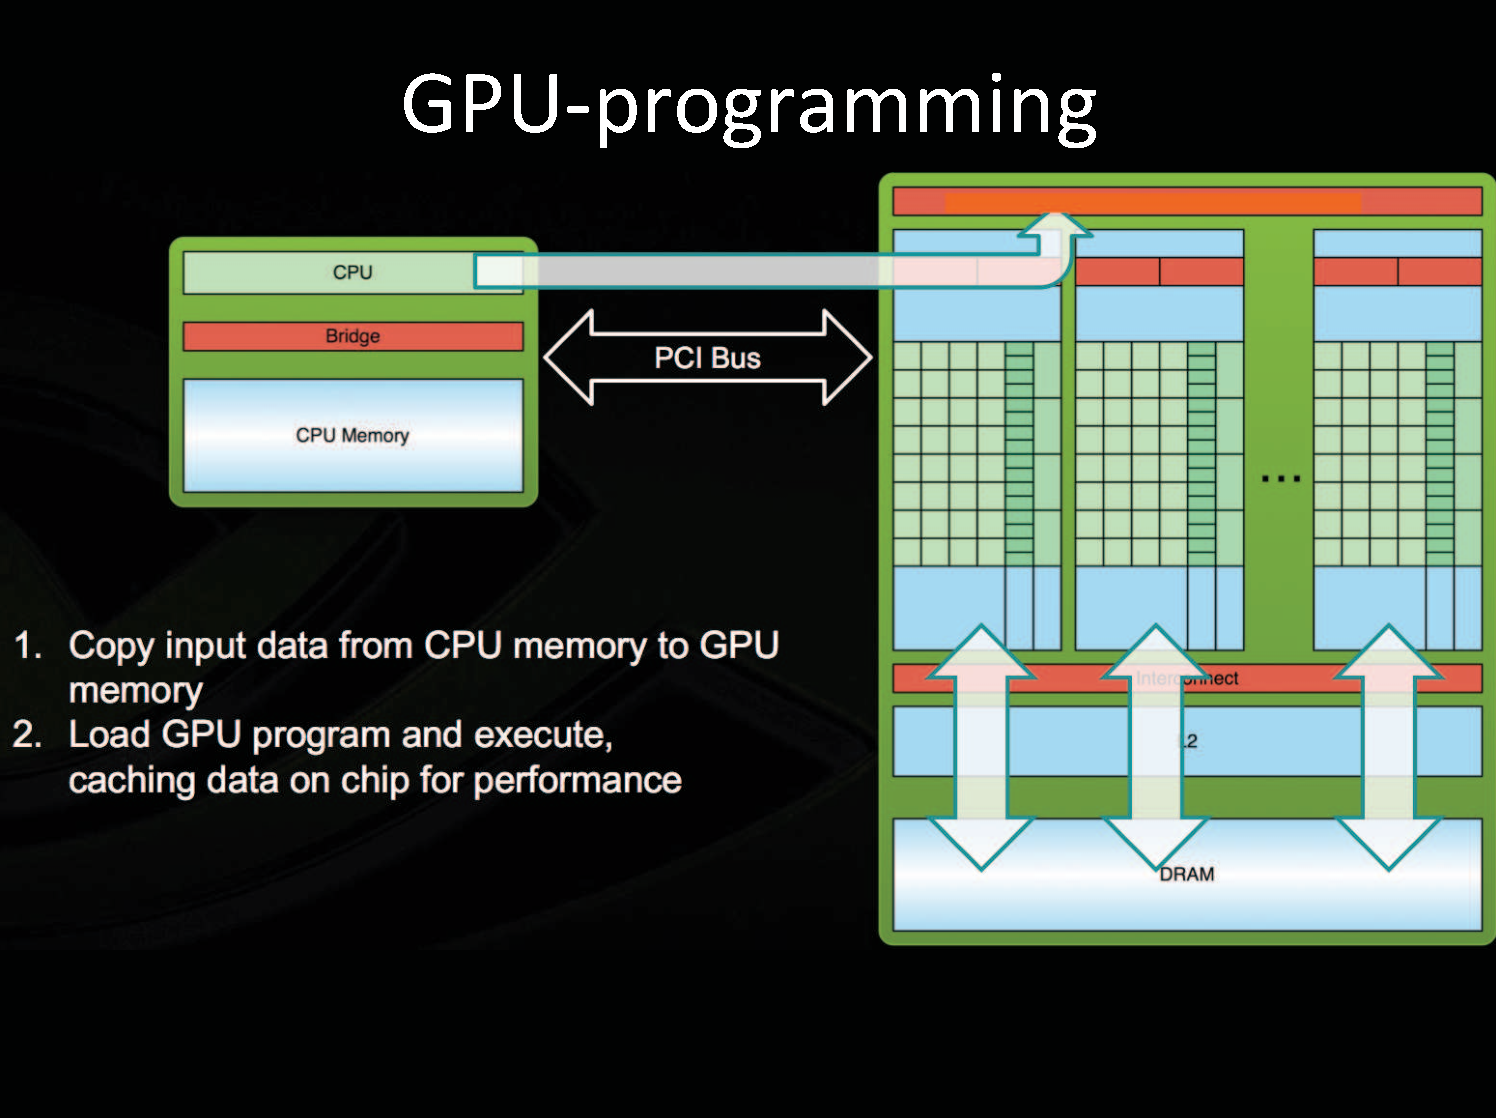
\includegraphics[height=43ex]{img/MemCpy2.pdf}
\end  {center}

\end{frame}


\begin{frame}[fragile,t]
\frametitle{GPU programming}

\begin{center}
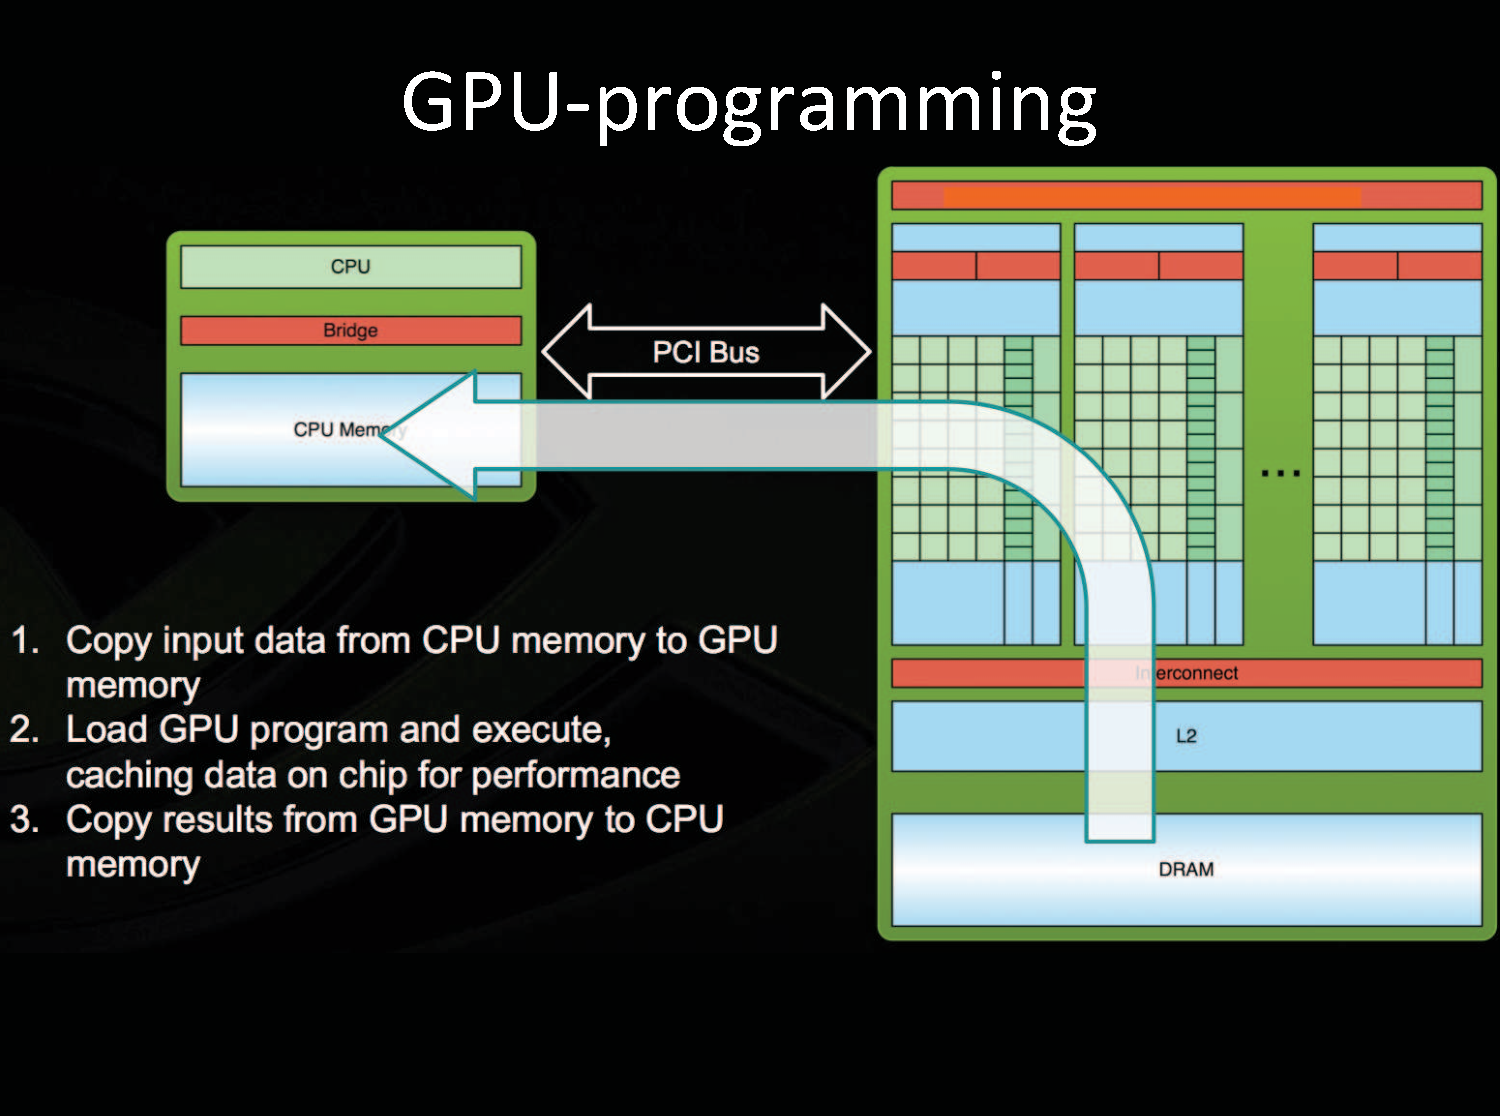
\includegraphics[height=43ex]{img/MemCpy3.pdf}
\end  {center}

\end{frame}

\begin{frame}
  \frametitle{OpenCL for this course}

  \begin{itemize}
  \item OpenCL is a standard C API for programming GPUs and other
    ``accelerators''.
  \item OpenCL is very low-level and very boilerplate-heavy.
  \item Any real application will build domain-specific abstraction
    layers on top.
  \item Since we want to teach you \textit{actual} OpenCL, we can't do
    that, but we will use a small library of abbreviations and
    helpers: \texttt{clutils.h}
  \item OpenCL comprises ordinary code running on the \textit{host}
    (CPU), which calls API functions to direct the \textit{device}
    (e.g. GPU).
  \end{itemize}

  \bigskip

  \hfill
\includegraphics[width=0.2\textwidth]{img/opencl-logo.png}

  \url{https://www.khronos.org/registry/OpenCL/sdk/1.0/docs/man/xhtml/}

\end{frame}

\begin{frame}
  \frametitle{OpenCL is an SIMT model}

  \textit{Single Instruction Multiple Threads} means we provide a
  \textit{sequential function} that is executed in parallel by
  multiple threads (``work items'' in OpenCL).

  \begin{center}
    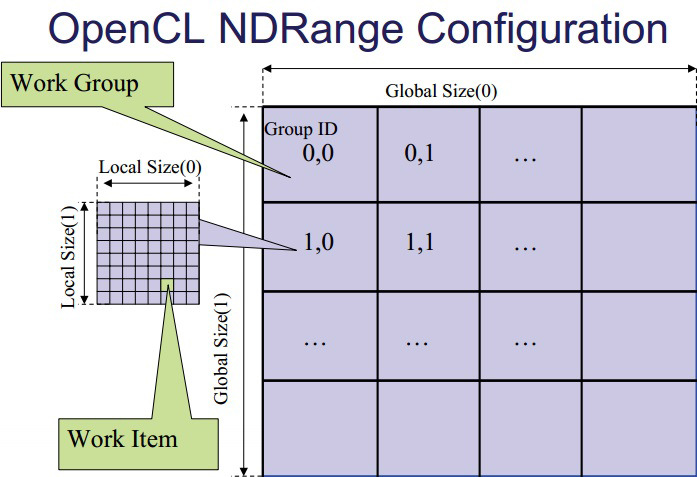
\includegraphics[width=0.75\textwidth]{img/ndrange.png}
  \end{center}

Threads are arranged in \textit{workgroups}, which form an
\textit{NDRange} (often called \textit{grid}).

\end{frame}

\begin{frame}
  \frametitle{OpenCL Platforms and Devices}

  A \textit{platform} is more like a \textit{vendor} (technically, an
  OpenCL backend or driver).  Each platform provides access to zero or
  more \textit{devices}.

  \begin{center}
    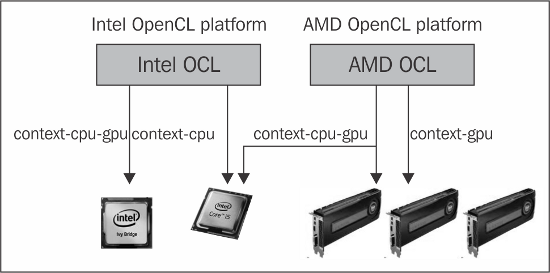
\includegraphics[width=\textwidth]{img/opencl-platforms-devices.png}
  \end{center}

  To use OpenCL, we must pick a \textit{platform}, then one of its
  \textit{devices}, use that to create a \textit{context}, and then a
  \textit{command queue} to which we can finally enqueue device
  operations.
\end{frame}

\begin{frame}[fragile,fragile]
  \frametitle{Listing available devices (Day1/devices.c)}

\begin{lstlisting}[backgroundcolor=\color{lightgray}]
cl_int clGetPlatformIDs
  (cl_uint num_entries,
   cl_platform_id *platforms,
   cl_uint *num_platforms)
\end{lstlisting}

\begin{lstlisting}
cl_uint num_platforms;

// Find the number of platforms.
OPENCL_SUCCEED(
  clGetPlatformIDs(0, NULL, &num_platforms));

printf("Found %d platforms\n",
       (int)num_platforms);
\end{lstlisting}

  The \texttt{OPENCL\_SUCCEED()} macro translates OpenCL error codes
  to strings and aborts the process in case of error.  Proper error
  handling is inherently application-specific and left as a very
  boring exercise.
\end{frame}

\begin{frame}[fragile]
\begin{lstlisting}
// Make room for them.
cl_platform_id *all_platforms =
  calloc(num_platforms, sizeof(cl_platform_id));

// Fetch all the platforms.
OPENCL_SUCCEED(
  clGetPlatformIDs(num_platforms,
                   all_platforms,
                   NULL));

for (unsigned int i = 0; i < num_platforms; i++) {
  ...
}
\end{lstlisting}
\end{frame}

\begin{frame}[fragile,fragile]
\begin{lstlisting}[backgroundcolor=\color{lightgray}]
cl_int clGetPlatformInfo
  (cl_platform_id platform,
   cl_platform_info param_name,
   size_t param_value_size,
   void *param_value,
   size_t *param_value_size_ret)
\end{lstlisting}

\begin{lstlisting}
size_t req_bytes;
char *name;

// How much space do we need for the platform name?
OPENCL_SUCCEED(
  clGetPlatformInfo(all_platforms[i],
                    CL_PLATFORM_NAME,
                    0, NULL,
                    &req_bytes));
\end{lstlisting}
\end{frame}

\begin{frame}[fragile]
\begin{lstlisting}
// Allocate space for the name and fetch it.
name = malloc(req_bytes);
OPENCL_SUCCEED(
  clGetPlatformInfo(all_platforms[i],
                    CL_PLATFORM_NAME,
                    req_bytes, name,
                    NULL));

printf("Platform %d: %s\n", i, name);

free(name);
\end{lstlisting}
\end{frame}

\begin{frame}[fragile]
\begin{lstlisting}
// Now let us print the names of all the devices,
// first we count how many of them exist.
cl_uint num_devices;
OPENCL_SUCCEED(
  clGetDeviceIDs(all_platforms[i],
                 CL_DEVICE_TYPE_ALL,
                 0, NULL,
                 &num_devices));

// Then we make room for them.
cl_device_id *platform_devices =
  calloc(num_devices, sizeof(cl_device_id));

// Then we fetch them.
OPENCL_SUCCEED(
  clGetDeviceIDs(all_platforms[i],
                 CL_DEVICE_TYPE_ALL,
                 num_devices, platform_devices,
                 NULL));
\end{lstlisting}
\end{frame}

\begin{frame}[fragile]
\begin{lstlisting}
for (unsigned int j = 0; j < num_devices; j++) {
  // How much space do we need for the device name?
  OPENCL_SUCCEED(
    clGetDeviceInfo(platform_devices[j],
                    CL_DEVICE_NAME,
                    0, NULL, &req_bytes));

  // Allocate space for the name and fetch it.
  name = malloc(req_bytes);
  OPENCL_SUCCEED(
    clGetDeviceInfo(platform_devices[j],
                    CL_DEVICE_NAME,
                    req_bytes, name, NULL));

  printf("\tDevice %d: %s\n", j, name);
  free(name);
}
\end{lstlisting}
\end{frame}

\begin{frame}[fragile]
  \frametitle{OpenCL in Visual Studio}

  \begin{block}{Warning}
    Neither Cosmin nor I are Windows users and we are entirely
    unexperienced with Visual Studio.
  \end{block}

  \begin{itemize}
  \item Ensure the AMD OpenCL SDK is installed.
  \item After creating a new project, edit its properties and set...
    \begin{enumerate}
    \item \textit{C/C++$\rightarrow$SDL checks} to No.
    \item \textit{C/C++$\rightarrow$Additional Include Directories}
      add \verb!C:\Program Files (x86)\AMD APP SDK\3.0\include!.
    \item \textit{Linker$\rightarrow$Additional Library Directories}
      add \verb!C:\Program Files (x86)\AMD APP SDK\3.0\lib!.
    \item \textit{Linker$\rightarrow$Input$\rightarrow$Additional
        Dependencies} add \verb!OpenCL.lib!.
    \end{enumerate}
  \item All but step 1 can be done by using the
    \texttt{AMDOpenCL.props} property sheet in the Git repository.
  \item Make sure you are doing a 64-bit build (VS calls this
    ``x64'').
  \end{itemize}

\end{frame}

\begin{frame}[fragile]
  \frametitle{Obtaining a \texttt{cl\_command\_queue} (clutils.h)}

Assuming variables \texttt{platform\_index} and \texttt{device\_index}.

\begin{lstlisting}
cl_uint num_platforms;
OPENCL_SUCCEED(
  clGetPlatformIDs(0, NULL, &num_platforms));
cl_platform_id *all_platforms =
  (cl_platform_id*)
  calloc(num_platforms, sizeof(cl_platform_id));
OPENCL_SUCCEED(
  clGetPlatformIDs(num_platforms,
                   all_platforms,
                   NULL));

assert(platform_index < num_platforms);
cl_platform_id platform =
  all_platforms[platform_index];
\end{lstlisting}

\end{frame}

\begin{frame}[fragile]
\begin{lstlisting}
cl_uint num_devices;
OPENCL_SUCCEED(
  clGetDeviceIDs(platform,
                 CL_DEVICE_TYPE_ALL,
                 0, NULL,
                 &num_devices));
cl_device_id *platform_devices =
  (cl_device_id*)
  calloc(num_devices, sizeof(cl_device_id));
OPENCL_SUCCEED(
  clGetDeviceIDs(platform,
                 CL_DEVICE_TYPE_ALL,
                 num_devices,
                 platform_devices,
                 NULL));

assert(device_index < num_devices);
cl_device_id device = platform_devices[device_index];
\end{lstlisting}
\end{frame}

\begin{frame}[fragile]

\begin{lstlisting}[backgroundcolor=\color{lightgray}]
cl_context clCreateContext
  (cl_context_properties *properties,
   cl_uint num_devices,
   const cl_device_id *devices,
   void *pfn_notify (...),
   void *user_data,
   cl_int *errcode_ret)
\end{lstlisting}

\begin{lstlisting}
cl_context_properties properties[] = {
  CL_CONTEXT_PLATFORM,
  (cl_context_properties)platform,
  0
};

cl_int error;
cl_context ctx =
  clCreateContext(properties, 1, &device,
                  NULL, NULL, &error);
OPENCL_SUCCEED(error);
\end{lstlisting}
\end{frame}

\begin{frame}[fragile,fragile]

\begin{lstlisting}[backgroundcolor=\color{lightgray}]
cl_command_queue clCreateCommandQueue
  (cl_context context,
   cl_device_id device,
   cl_command_queue_properties properties,
   cl_int *errcode_ret)
\end{lstlisting}

\begin{lstlisting}
cl_command_queue queue =
  clCreateCommandQueue(*ctx, *device, 0, &error);
OPENCL_SUCCEED(error);
\end{lstlisting}

  Using \texttt{clutils.h}, all of the above can be replaced with:

\begin{lstlisting}
cl_context ctx;
cl_command_queue queue;
cl_device_id device;
opencl_init_command_queue_default
  (&device, &ctx, &queue);
\end{lstlisting}

\end{frame}

\begin{frame}[fragile]
  \frametitle{Rot-13 in OpenCL (Day1/rot13.c)}

Rot-13 is a cutting edge encryption algorithm.  In C, it is:

\begin{lstlisting}
void rot13(char *out, char *in, int n) {
  for (int i = 0; i < n; i++) {
    if (i < n) {
      if (in[i] >= 'a' && in[i] <= 'z') {
        out[i] = (in[i] - 'a' + 13) % 26 + 'a';
      } else {
        out[i] = in[i];
      }
    }
  }
}
\end{lstlisting}

Here restricted to operate on lowercase ASCII only to ensure readable
output.

\end{frame}

\begin{frame}[fragile]
  \frametitle{Loading OpenCL programs}

  We obtain an OpenCL \textit{program} by passing its source (written
  in OpenCL C) to \texttt{clBuildProgram()}.  Lots of boilerplate
  again; let's just use \texttt{clutils.h}:

\begin{lstlisting}
cl_program program =
  opencl_build_program(ctx, device,
                       "kernels/rot13.cl",
                       "");
\end{lstlisting}

  OpenCL C is a cut-down dialect of C with many restrictions:

  \begin{itemize}
  \item No function pointers.
  \item No recursion.
  \item Limited standard library.
  \item No memory allocation.
  \item No printing to the screen.
  \item \textit{Etc...}
  \end{itemize}
\end{frame}

\begin{frame}[fragile]
  \frametitle{Kernel functions (Day1/kernels/rot13.cl)}

  An OpenCL C program contains kernel functions that serve as
  entry points:

\begin{lstlisting}
// Rot-13 for lowercase ASCII.
kernel void rot13(global char *out,
                  global char *in,
                  int n) {
  int gtid = get_global_id(0);
  if (gtid < n) {
    if (in[gtid] >= 'a' &&
        in[gtid] <= 'z') {
      out[gtid] = (in[gtid] - 'a' + 13)
                  % 26 + 'a';
    } else {
      out[gtid] = in[gtid];
    }
  }
}
\end{lstlisting}
\end{frame}

\begin{frame}[fragile]
  \frametitle{Accesing kernels (Day1/rot13.c)}

  To launch a kernel on the GPU from the host, we first use
  \texttt{clCreateKernel()} with the \texttt{cl\_program} object we
  got back:

\begin{lstlisting}
cl_kernel rot13_k =
  clCreateKernel(program, "rot13", &error);
OPENCL_SUCCEED(error);
\end{lstlisting}

  \begin{itemize}
  \item Now we can ask the GPU to run the kernel.
  \item Except that GPUs have their own separate memory, so we have no
    data for the kernel to work on!
  \end{itemize}

\end{frame}

\begin{frame}[fragile,fragile]
  \frametitle{Allocating GPU memory}

\begin{lstlisting}[backgroundcolor=\color{lightgray}]
cl_mem clCreateBuffer(cl_context context,
                      cl_mem_flags flags,
                      size_t size,
                      void *host_ptr,
                      cl_int *errcode_ret)
\end{lstlisting}

\begin{lstlisting}
char *string = "Hello, World!\n";
cl_int n = strlen(string);

cl_mem input =
   clCreateBuffer(ctx,
                  CL_MEM_READ_ONLY
                  | CL_MEM_COPY_HOST_PTR,
                  n, string, &error);

cl_mem output =
  clCreateBuffer(ctx, CL_MEM_WRITE_ONLY,
                 n, NULL, &error);
\end{lstlisting}

\end{frame}

\begin{frame}[fragile,fragile]
  \frametitle{Passing arguments to the kernel}

  Remember that \texttt{rot13\_k} object?  We finally get to use it.

\begin{lstlisting}
clSetKernelArg
  (rot13_k, 0, sizeof(cl_mem), &output);
clSetKernelArg
  (rot13_k, 1, sizeof(cl_mem), &input);
clSetKernelArg
  (rot13_k, 2, sizeof(cl_int), &n);
\end{lstlisting}

Reminder on \texttt{Day1/kernels/rot13.cl}:

\begin{lstlisting}
kernel void rot13(global char *out,
                  global char *in,
                  int n) {
  ...
}
\end{lstlisting}

\end{frame}

\begin{frame}[fragile]
  \frametitle{Launching a kernel}

  When launching a kernel, we must specify the layout of the grid:

  \begin{itemize}
  \item The number of dimensions (1, 2, or 3).
  \item The size of each workgroup in each dimension.
  \item The total number of threads in each dimension (which must be
    divisible by the workgroup size in that dimension).
  \end{itemize}

  For our rot-13, we want a 1D grid with one thread per input, rounded
  up to the workgroup size.

\begin{lstlisting}
size_t local_work_size[1] = { 256 };
size_t global_work_size[1] = {
  div_rounding_up(n, local_work_size[0])
  * local_work_size[0]
};
\end{lstlisting}

Workgroup size is a tunable parameter, but we'll always pick 256 for
now.

\end{frame}

\begin{frame}[fragile,fragile]
  \frametitle{\texttt{clEnqueueNDRangeKernel()}}

\begin{lstlisting}[backgroundcolor=\color{lightgray}]
cl_int clEnqueueNDRangeKernel
  (cl_command_queue command_queue,
   cl_kernel kernel,
   cl_uint work_dim,
   const size_t *global_work_offset,
   const size_t *global_work_size,
   const size_t *local_work_size,
   cl_uint num_events_in_wait_list,
   const cl_event *event_wait_list,
   cl_event *event)
\end{lstlisting}

\begin{lstlisting}
clEnqueueNDRangeKernel(queue, rot13_k,
                       1,
                       NULL,
                       global_work_size,
                       local_work_size,
                       0, NULL, NULL);
\end{lstlisting}

\end{frame}

\begin{frame}[fragile]
  \frametitle{More on command queues}

  \begin{itemize}
  \item Enqueuing a command is \textit{asynchronous}.  It might start
    executing immediately, soon, or not at all.
  \item Use \texttt{clFinish()} to ensure that all operations have
    finished:
  \end{itemize}

\begin{lstlisting}
OPENCL_SUCCEED(clFinish(queue));
\end{lstlisting}

  This is also where execution errors are typically reported.
\end{frame}

\begin{frame}[fragile]
  \frametitle{Reading results back from the GPU}

\begin{lstlisting}[backgroundcolor=\color{lightgray}]
cl_int clEnqueueReadBuffer
  (cl_command_queue command_queue,
   cl_mem buffer,
   cl_bool blocking_read,
   size_t offset, size_t cb, void *ptr,
   cl_uint num_events_in_wait_list,
   const cl_event *event_wait_list,
   cl_event *event)
\end{lstlisting}

\begin{lstlisting}
char *output_string = malloc(n + 1);
output_string[n] = '\0'; // Ensure 0-termination.
clEnqueueReadBuffer(queue, output, CL_TRUE,
                    0, n,
                    output_string,
                    0, NULL, NULL);

printf("Result: %s\n", output_string);
\end{lstlisting}

\end{frame}

\section{Debugging and Profiling OpenCL}

\begin{frame}
	\tableofcontents[currentsection]
\end{frame}

\begin{frame}[fragile]
  \frametitle{Debugging with \texttt{oclgrind}}

  \begin{itemize}
  \item \url{https://github.com/jrprice/Oclgrind}
  \item Makes itself available as an OpenCL platform that runs your
    kernels in an error-checking interpreter.
  \item A lot like \texttt{valgrind}.
  \item Fairly slow, so use it on reduced workloads.
  \end{itemize}

\begin{lstlisting}[basicstyle=\small,breaklines=true]
$ oclgrind ./rot13
Using platform: Oclgrind
Using device: Oclgrind Simulator

Invalid read of size 1 at global memory address 0x100000000000e
  Kernel: rot13
  Entity: Global(14,0,0) Local(14,0,0) Group(0,0,0)
    %1 = load i8, i8 addrspace(1)* %arrayidx, align 1, !dbg !20
  At line 5 of input.cl:
    if (in[gtid] >= 'a' && in[gtid] <= 'z') {
...
\end{lstlisting}

\end{frame}

\begin{frame}[fragile]
  \frametitle{Profiling with Wall Clock Time}

Just like how you profile anything else.

\begin{lstlisting}
// Current wall time in microseconds.
static int64_t get_wall_time(void);
\end{lstlisting}

Use it like this:

\begin{lstlisting}
int64_t before = get_wall_time();

...

clFinish(ctx);

int64_t after = get_wall_time();

printf("Took %d microseconds\n",
       (int)(after-before));
\end{lstlisting}

The \lstinline{clFinish()} call is crucial as otherwise the device may
still be working (remember that most enqueuings are
\textit{asynchronous}).

\end{frame}

\begin{frame}[fragile]
  \frametitle{Profiling with Events}

  An event is an object that communicates the status of an OpenCL
  command.  Whenever we enqueue something in a command queue, we can
  get an event object back.

\begin{lstlisting}[backgroundcolor=\color{lightgray}]
 cl_int clEnqueueNDRangeKernel
   (cl_command_queue command_queue,
    cl_kernel kernel,
    cl_uint work_dim,
    const size_t *global_work_offset,
    const size_t *global_work_size,
    const size_t *local_work_size,
    cl_uint num_events_in_wait_list,
    const cl_event *event_wait_list,
    @cl_event *event@)
\end{lstlisting}

\end{frame}

\begin{frame}[fragile]
  \frametitle{Retrieving Information from Events}

\begin{lstlisting}[backgroundcolor=\color{lightgray}]
cl_int clGetEventInfo
  (cl_event event,
   cl_event_info param_name,
   size_t param_value_size,
   void *param_value,
   size_t *param_value_size_ret)
\end{lstlisting}

\begin{lstlisting}
 cl_int clGetEventProfilingInfo
   (cl_event event,
    cl_profiling_info param_name,
    size_t param_value_size,
    void *param_value,
    size_t *param_value_size_ret)
\end{lstlisting}

  The latter only works if \lstinline{CL_QUEUE_PROFILING_ENABLE} was
  passed to \lstinline{clCreateCommandQueue()}.
\end{frame}

\begin{frame}[fragile]
  \frametitle{Values for \texttt{cl\_profiling\_info}}

  \begin{description}
  \item[\texttt{CL\_PROFILING\_COMMAND\_QUEUED}]\hfill\\ When the
    command was queued.
  \item[\texttt{CL\_PROFILING\_COMMAND\_SUBMIT}]\hfill\\ When the
    command was sent to the device.
  \item[\texttt{CL\_PROFILING\_COMMAND\_START}]\hfill\\ When the
    command started executing.
  \item[\texttt{CL\_PROFILING\_COMMAND\_END}]\hfill\\ When the
    command finished executing.
  \end{description}

  \begin{itemize}
  \item All produce a value of type \lstinline{cl_ulong}.
  \item \lstinline{clGetEventProfilingInfo()} returns
    \lstinline{CL_PROFILING_INFO_NOT_AVAILABLE} if the information is
    not available (yet)
  \end{itemize}
\end{frame}

\begin{frame}[fragile]
  \frametitle{Example of Profiling with Events}

\begin{lstlisting}
cl_event write_e;
clEnqueueWriteBuffer(queue, to, CL_FALSE,
                     0, n,
                     from,
                     0, NULL, &write_e));

...

cl_ulong start, end;

clGetEventProfilingInfo
  (write_e, CL_PROFILING_COMMAND_START,
   sizeof(start), &start, NULL);
clGetEventProfilingInfo
  (write_e, CL_PROFILING_COMMAND_START,
   sizeof(end), &end, NULL);
\end{lstlisting}

\end{frame}

\begin{frame}
  \frametitle{Event Profiling versus Wall Clock Profiling}

  \begin{itemize}
  \item Event profiling is \textbf{much more fine-grained} and lets us
    see the per-operation runtime.
  \item Measuring per-operation with wall clock would require us to
    \texttt{clFinish()} after every operation, which is very slow
    because it prevents pipelining.
  \item Wall clock profiling tells us about \textbf{overall
      application performance}.  We generally cannot just sum the
    runtimes for each event, since the commands may overlap in time,
    and the events do not count host-based overheads.
  \item \textbf{Ideally, use both.}
  \end{itemize}

  However, neither of these approaches will tell us \textit{why}
  something is slow...
\end{frame}

\section{Coalesced Memory Accesses}

\begin{frame}
	\tableofcontents[currentsection]
\end{frame}

\begin{frame}[fragile]
  \frametitle{Summing the rows of a matrix}

  Consider summing the rows/columns of a $10000\times{}10000$
  row-major matrix on CPU and GPU:

  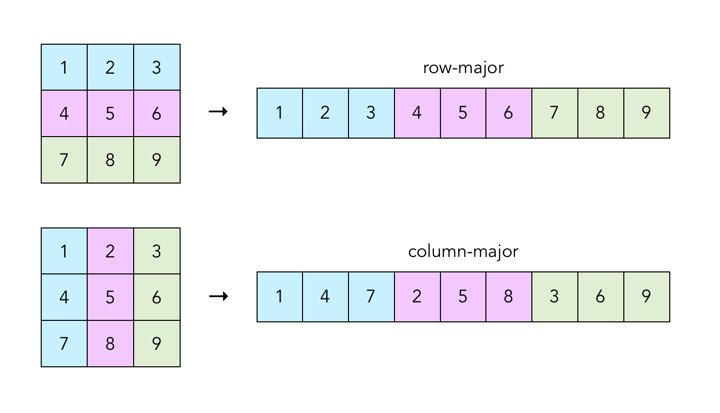
\includegraphics[width=\textwidth]{img/rowcolumnarrays.jpg}

\end{frame}

\begin{frame}[fragile]
  \frametitle{Performance}

\begin{lstlisting}
for (int row = 0; row < n; row++) {
  cl_int sum = 0;
  for (int col = 0; col < n; col++) {
    sum += matrix[row*n+col];
  }
  sums[row] = sum;
}
\end{lstlisting}

On the GPU, we assign one iteration of the outer loop to each thread.

\bigskip

  \begin{tabular}{lr}
    Summing rows on CPU & $22025\mu{}s$ \\
    Summing columns on CPU & $741225\mu{}s$ \\
    Summing rows on GPU & $60461\mu{}s$ \\
    Summing columns on GPU & $6169\mu{}s$
  \end{tabular}

\end{frame}

\begin{frame}
  \frametitle{Why does this go so badly?}

  The reason is our memory access pattern -- specifically, our loads
  are not \textit{coalesced}.

  \begin{block}{Memory Coalescing}
    All threads within each consecutive 16-thread gang should
    simultaneously access consecutive elements in memory to maximise
    memory bus usage.
  \end{block}

  \begin{itemize}
  \item If neighboring threads access widely distant memory in the same
    clock cycle, the loads have to be \textit{sequentialised}, instead
    of all fulfilled using one (wide) memory bus operation.
  \item The HD 7800 has a memory bus width of 256 bits, so only using
    32 bits per operation exploits an eight of the bandwidth.
  \end{itemize}

\end{frame}

\begin{frame}
  \frametitle{The accesses specifically}

\begin{table}[H]
\caption{Current accesses - this is worst case behaviour!}
  \begin{tabular}{l|llll}
    \textbf{Iteration} & \textbf{Thread $0$} & \textbf{Thread $1$} & \textbf{Thread $2$} & ... \\\hline
    0 & $\texttt{matrix}[0]$ & $\texttt{matrix}[n]$ & $\texttt{matrix}[2n]$ & ... \\
    1 & $\texttt{matrix}[1]$ & $\texttt{matrix}[n+1]$ & $\texttt{matrix}[2n+1]$ & ... \\
    2 & $\texttt{matrix}[2]$ & $\texttt{matrix}[n+2]$ & $\texttt{matrix}[2n+2]$ & ... \\
  \end{tabular}
\end{table}

\begin{table}[H]
\caption{These are the accesses we want}
  \begin{tabular}{l|llll}
    \textbf{Iteration} & \textbf{Thread $0$} & \textbf{Thread $1$} & \textbf{Thread $2$} & ... \\\hline
    0 & $\texttt{matrix}[0]$ & $\texttt{matrix}[1]$ & $\texttt{matrix}[2]$ & ... \\
    1 & $\texttt{matrix}[n]$ & $\texttt{matrix}[n+1]$ & $\texttt{matrix}[n+2]$ & ... \\
    2 & $\texttt{matrix}[nc]$ & $\texttt{matrix}[2n+1]$ & $\texttt{matrix}[2n+2]$ & ... \\
  \end{tabular}
\end{table}

\textit{This is the exact opposite of what we are usually taught for
  CPUs!}

\end{frame}

\section{Programming Exercises}

\begin{frame}
	\tableofcontents[currentsection]
\end{frame}

\begin{frame}
  \frametitle{Profiling rot-13 with wall clock and events}

  \begin{itemize}
  \item \texttt{Day1-exercises/rot13-profile-simple.c}
  \item \texttt{Day1-exercises/rot13-profile-events.c}
  \end{itemize}

  Try profiling both one and multiple kernel launches.  What do you
  observe?  What if you call \texttt{clFinish()} after every kernel
  invocation?  What if you also count the cost of copying from the CPU
  to the GPU?

\end{frame}

\begin{frame}
  \frametitle{Reversing a string in parallel}

  Write an OpenCL for reversing a string.  Base it heavily on the
  Rot-13 program.  Create your own Visual Studio project for it as
  well.
\end{frame}

\begin{frame}[fragile]
  \frametitle{Load balancing (\texttt{Day1-exercises/fibfact.c})}

  Finish the program, which is supposed to do the equivalent of:

\begin{lstlisting}
void f (int k, float *out, int *ns, int *op)
for (int i = 0; i < k; i++) {
  int n = ns[i];
  int x;
  if (op[i] == 1) {
    x = fib(n);
  } else {
    x = fact(n);
  }
  out[i] = x;
}
\end{lstlisting}

  \begin{itemize}
  \item Where \texttt{fact()} and \texttt{fib()} are the usual
    factorial and Fibonacci functions.
  \item How fast does it run for various contents of \texttt{ns} and
    \texttt{ops}?  Can you make it faster by preprocessing these
    arrays?
  \end{itemize}

\end{frame}

\begin{frame}
  \frametitle{Implementing Game of Life (\texttt{Day1-exercises/life-arrays.c})}

  Conway's Game of Life is a simple 2D cellular automaton
  (``stencil'') that is embarassingly parallel.  Each cell is updated
  based on the value of its neighbours.

  \begin{center}
    
\includegraphics[width=4cm]{img/stencil.png}
  \end{center}

\end{frame}

\begin{frame}
  \frametitle{Using image objects for Game of Life (\texttt{Day1-exercises/life-images.c})}

  \begin{itemize}
  \item GPUs have special hardware for textures, and this can be used
    whenever we need 2D arrays with spatial locality (like in Game of
    Life).

  \item Instead of \texttt{clCreateBuffer()}, use
    \texttt{clCreateImage()}, and in the kernel use the
    \texttt{image2d\_t} type.

  \item Implement this as a 2D kernel in
    \texttt{Day1-exercises/life-images.c}.

  \item Main challenge: understand the OpenCL documentation and figure
    out how to represent our information in a colour channel.
  \end{itemize}
\end{frame}

\begin{frame}[fragile,fragile,fragile]
  \frametitle{Help for image objects}

\begin{lstlisting}[backgroundcolor=\color{lightgray}]
cl_mem clCreateImage
  (cl_context context,
   cl_mem_flags flags,
   const cl_image_format *image_format,
   const cl_image_desc *image_desc,
   void *host_ptr,
   cl_int *errcode_ret)
\end{lstlisting}

  This is probably the best image format for us:

\begin{lstlisting}
cl_image_format format =
  { .image_channel_order = CL_RGBA,
    .image_channel_data_type = CL_UNSIGNED_INT8
  };
\end{lstlisting}

\end{frame}

\begin{frame}[fragile]
  \frametitle{Image objects inside kernels}

Inside the kernel we can use these functions to read/write elements:

\begin{lstlisting}
unsigned int4 read_imageui(image2d_t image,
                           sampler_t sampler,
                           int2 coord)

void write_imageui(image2d_t image,
                   int2 coord,
                   unsigned int4 color)
\end{lstlisting}

E.g.

\begin{lstlisting}
write_imageui(img,
              (int2)(x,y),
              (uint4)(r,g,b,a))
uint4 v = read_imageui(img, sampler, (int2)(x,y));
// v.s0, v.s1, v.s2, v.s3
\end{lstlisting}

\end{frame}

\begin{frame}
  \frametitle{Matrix multiplication}

  \begin{itemize}
  \item Implement matrix multiplication as a 2D kernel with one thread
    per element of the output matrix.
  \item \textbf{Spoiler alert:} you will find that it is slow.  Why?
  \end{itemize}

  Cosmin will eventually tell you how to make it less slow.

\end{frame}

\end{document}

%%% Local Variables:
%%% mode: latex
%%% TeX-master: t
%%% End:
